% Options for packages loaded elsewhere
\PassOptionsToPackage{unicode}{hyperref}
\PassOptionsToPackage{hyphens}{url}
%
\documentclass[
  ignorenonframetext,
]{beamer}
\usepackage{pgfpages}
\setbeamertemplate{caption}[numbered]
\setbeamertemplate{caption label separator}{: }
\setbeamercolor{caption name}{fg=normal text.fg}
\beamertemplatenavigationsymbolshorizontal
% Prevent slide breaks in the middle of a paragraph
\widowpenalties 1 10000
\raggedbottom
\setbeamertemplate{part page}{
  \centering
  \begin{beamercolorbox}[sep=16pt,center]{part title}
    \usebeamerfont{part title}\insertpart\par
  \end{beamercolorbox}
}
\setbeamertemplate{section page}{
  \centering
  \begin{beamercolorbox}[sep=12pt,center]{part title}
    \usebeamerfont{section title}\insertsection\par
  \end{beamercolorbox}
}
\setbeamertemplate{subsection page}{
  \centering
  \begin{beamercolorbox}[sep=8pt,center]{part title}
    \usebeamerfont{subsection title}\insertsubsection\par
  \end{beamercolorbox}
}
\AtBeginPart{
  \frame{\partpage}
}
\AtBeginSection{
  \ifbibliography
  \else
    \frame{\sectionpage}
  \fi
}
\AtBeginSubsection{
  \frame{\subsectionpage}
}

\usepackage{amsmath,amssymb}
\usepackage{iftex}
\ifPDFTeX
  \usepackage[T1]{fontenc}
  \usepackage[utf8]{inputenc}
  \usepackage{textcomp} % provide euro and other symbols
\else % if luatex or xetex
  \usepackage{unicode-math}
  \defaultfontfeatures{Scale=MatchLowercase}
  \defaultfontfeatures[\rmfamily]{Ligatures=TeX,Scale=1}
\fi
\usepackage{lmodern}
\usetheme[]{default}
\ifPDFTeX\else  
    % xetex/luatex font selection
\fi
% Use upquote if available, for straight quotes in verbatim environments
\IfFileExists{upquote.sty}{\usepackage{upquote}}{}
\IfFileExists{microtype.sty}{% use microtype if available
  \usepackage[]{microtype}
  \UseMicrotypeSet[protrusion]{basicmath} % disable protrusion for tt fonts
}{}
\makeatletter
\@ifundefined{KOMAClassName}{% if non-KOMA class
  \IfFileExists{parskip.sty}{%
    \usepackage{parskip}
  }{% else
    \setlength{\parindent}{0pt}
    \setlength{\parskip}{6pt plus 2pt minus 1pt}}
}{% if KOMA class
  \KOMAoptions{parskip=half}}
\makeatother
\usepackage{xcolor}
\newif\ifbibliography
\usepackage{svg}
\setlength{\emergencystretch}{3em} % prevent overfull lines
\setcounter{secnumdepth}{-\maxdimen} % remove section numbering

\usepackage{color}
\usepackage{fancyvrb}
\newcommand{\VerbBar}{|}
\newcommand{\VERB}{\Verb[commandchars=\\\{\}]}
\DefineVerbatimEnvironment{Highlighting}{Verbatim}{commandchars=\\\{\}}
% Add ',fontsize=\small' for more characters per line
\usepackage{framed}
\definecolor{shadecolor}{RGB}{241,243,245}
\newenvironment{Shaded}{\begin{snugshade}}{\end{snugshade}}
\newcommand{\AlertTok}[1]{\textcolor[rgb]{0.68,0.00,0.00}{#1}}
\newcommand{\AnnotationTok}[1]{\textcolor[rgb]{0.37,0.37,0.37}{#1}}
\newcommand{\AttributeTok}[1]{\textcolor[rgb]{0.40,0.45,0.13}{#1}}
\newcommand{\BaseNTok}[1]{\textcolor[rgb]{0.68,0.00,0.00}{#1}}
\newcommand{\BuiltInTok}[1]{\textcolor[rgb]{0.00,0.23,0.31}{#1}}
\newcommand{\CharTok}[1]{\textcolor[rgb]{0.13,0.47,0.30}{#1}}
\newcommand{\CommentTok}[1]{\textcolor[rgb]{0.37,0.37,0.37}{#1}}
\newcommand{\CommentVarTok}[1]{\textcolor[rgb]{0.37,0.37,0.37}{\textit{#1}}}
\newcommand{\ConstantTok}[1]{\textcolor[rgb]{0.56,0.35,0.01}{#1}}
\newcommand{\ControlFlowTok}[1]{\textcolor[rgb]{0.00,0.23,0.31}{\textbf{#1}}}
\newcommand{\DataTypeTok}[1]{\textcolor[rgb]{0.68,0.00,0.00}{#1}}
\newcommand{\DecValTok}[1]{\textcolor[rgb]{0.68,0.00,0.00}{#1}}
\newcommand{\DocumentationTok}[1]{\textcolor[rgb]{0.37,0.37,0.37}{\textit{#1}}}
\newcommand{\ErrorTok}[1]{\textcolor[rgb]{0.68,0.00,0.00}{#1}}
\newcommand{\ExtensionTok}[1]{\textcolor[rgb]{0.00,0.23,0.31}{#1}}
\newcommand{\FloatTok}[1]{\textcolor[rgb]{0.68,0.00,0.00}{#1}}
\newcommand{\FunctionTok}[1]{\textcolor[rgb]{0.28,0.35,0.67}{#1}}
\newcommand{\ImportTok}[1]{\textcolor[rgb]{0.00,0.46,0.62}{#1}}
\newcommand{\InformationTok}[1]{\textcolor[rgb]{0.37,0.37,0.37}{#1}}
\newcommand{\KeywordTok}[1]{\textcolor[rgb]{0.00,0.23,0.31}{\textbf{#1}}}
\newcommand{\NormalTok}[1]{\textcolor[rgb]{0.00,0.23,0.31}{#1}}
\newcommand{\OperatorTok}[1]{\textcolor[rgb]{0.37,0.37,0.37}{#1}}
\newcommand{\OtherTok}[1]{\textcolor[rgb]{0.00,0.23,0.31}{#1}}
\newcommand{\PreprocessorTok}[1]{\textcolor[rgb]{0.68,0.00,0.00}{#1}}
\newcommand{\RegionMarkerTok}[1]{\textcolor[rgb]{0.00,0.23,0.31}{#1}}
\newcommand{\SpecialCharTok}[1]{\textcolor[rgb]{0.37,0.37,0.37}{#1}}
\newcommand{\SpecialStringTok}[1]{\textcolor[rgb]{0.13,0.47,0.30}{#1}}
\newcommand{\StringTok}[1]{\textcolor[rgb]{0.13,0.47,0.30}{#1}}
\newcommand{\VariableTok}[1]{\textcolor[rgb]{0.07,0.07,0.07}{#1}}
\newcommand{\VerbatimStringTok}[1]{\textcolor[rgb]{0.13,0.47,0.30}{#1}}
\newcommand{\WarningTok}[1]{\textcolor[rgb]{0.37,0.37,0.37}{\textit{#1}}}

\providecommand{\tightlist}{%
  \setlength{\itemsep}{0pt}\setlength{\parskip}{0pt}}\usepackage{longtable,booktabs,array}
\usepackage{calc} % for calculating minipage widths
\usepackage{caption}
% Make caption package work with longtable
\makeatletter
\def\fnum@table{\tablename~\thetable}
\makeatother
\usepackage{graphicx}
\makeatletter
\def\maxwidth{\ifdim\Gin@nat@width>\linewidth\linewidth\else\Gin@nat@width\fi}
\def\maxheight{\ifdim\Gin@nat@height>\textheight\textheight\else\Gin@nat@height\fi}
\makeatother
% Scale images if necessary, so that they will not overflow the page
% margins by default, and it is still possible to overwrite the defaults
% using explicit options in \includegraphics[width, height, ...]{}
\setkeys{Gin}{width=\maxwidth,height=\maxheight,keepaspectratio}
% Set default figure placement to htbp
\makeatletter
\def\fps@figure{htbp}
\makeatother

\usepackage{fontspec}
\usepackage{graphicx}
\usepackage{grffile}
\makeatletter
\@ifpackageloaded{caption}{}{\usepackage{caption}}
\AtBeginDocument{%
\ifdefined\contentsname
  \renewcommand*\contentsname{Table of contents}
\else
  \newcommand\contentsname{Table of contents}
\fi
\ifdefined\listfigurename
  \renewcommand*\listfigurename{List of Figures}
\else
  \newcommand\listfigurename{List of Figures}
\fi
\ifdefined\listtablename
  \renewcommand*\listtablename{List of Tables}
\else
  \newcommand\listtablename{List of Tables}
\fi
\ifdefined\figurename
  \renewcommand*\figurename{Figure}
\else
  \newcommand\figurename{Figure}
\fi
\ifdefined\tablename
  \renewcommand*\tablename{Table}
\else
  \newcommand\tablename{Table}
\fi
}
\@ifpackageloaded{float}{}{\usepackage{float}}
\floatstyle{ruled}
\@ifundefined{c@chapter}{\newfloat{codelisting}{h}{lop}}{\newfloat{codelisting}{h}{lop}[chapter]}
\floatname{codelisting}{Listing}
\newcommand*\listoflistings{\listof{codelisting}{List of Listings}}
\makeatother
\makeatletter
\makeatother
\makeatletter
\@ifpackageloaded{caption}{}{\usepackage{caption}}
\@ifpackageloaded{subcaption}{}{\usepackage{subcaption}}
\makeatother

\ifLuaTeX
  \usepackage{selnolig}  % disable illegal ligatures
\fi
\usepackage{bookmark}

\IfFileExists{xurl.sty}{\usepackage{xurl}}{} % add URL line breaks if available
\urlstyle{same} % disable monospaced font for URLs
\hypersetup{
  pdftitle={Class 31},
  pdfauthor={Sarah E. Grabinski},
  hidelinks,
  pdfcreator={LaTeX via pandoc}}


\title{Class 31}
\subtitle{DATA1220-55, Fall 2024}
\author{Sarah E. Grabinski}
\date{2024-11-20}

\begin{document}
\frame{\titlepage}


\begin{frame}{Review: 2 Numeric Variables}
\phantomsection\label{review-2-numeric-variables}
\begin{center}
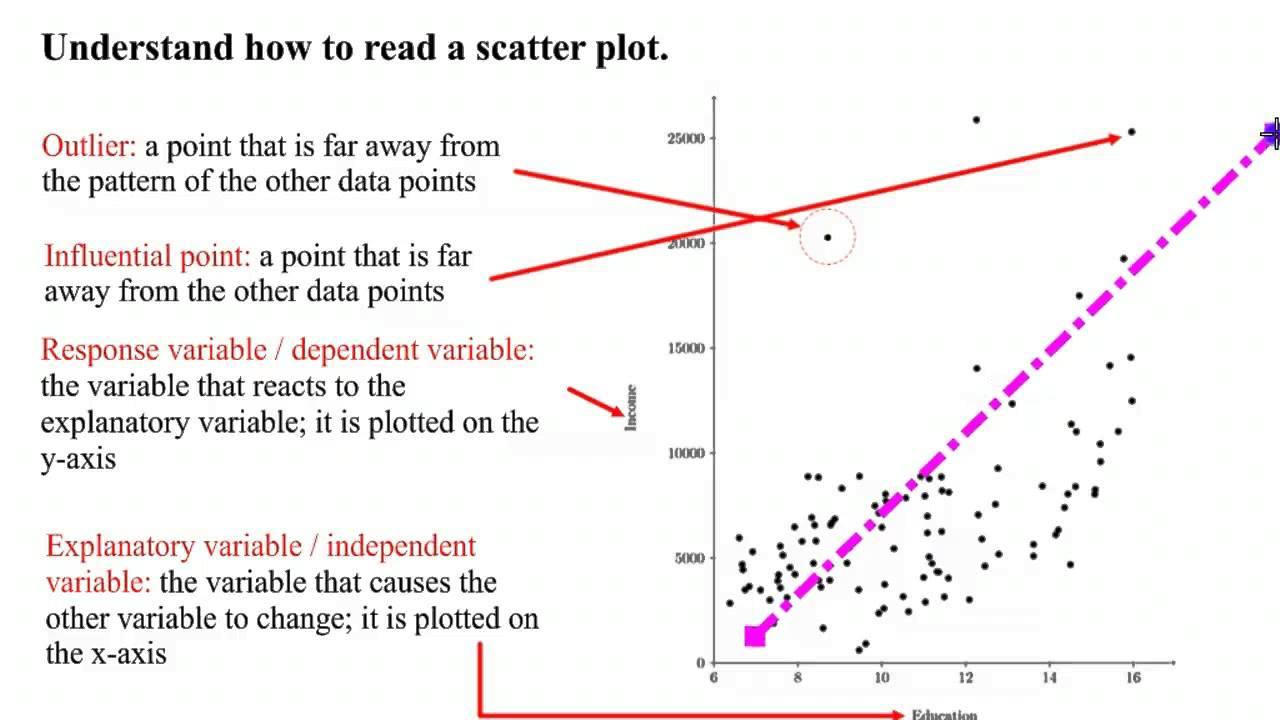
\includegraphics{class31_files/mediabag/scatter-plot-guide.jpg}
\end{center}
\end{frame}

\begin{frame}{Review: Describing Associations}
\phantomsection\label{review-describing-associations}
\begin{itemize}
\tightlist
\item
  \textbf{\emph{Independence}}: an increase in \(X\) is not associated
  with a change in \(Y\)
\end{itemize}

\pause

\begin{itemize}
\tightlist
\item
  \textbf{\emph{Positive association}}: an increase in \(X\) is
  associated with an \emph{increase} in \(Y\)
\end{itemize}

\pause

\begin{itemize}
\tightlist
\item
  \textbf{\emph{Negative association}}: an increase in \(X\) is
  associated with a \emph{decrease} in \(Y\)
\end{itemize}

\pause

\begin{itemize}
\tightlist
\item
  \textbf{\emph{Weak association}}: data points are very far apart from
  each other
\end{itemize}

\pause

\begin{itemize}
\tightlist
\item
  \textbf{\emph{Strong association}}: data points are tightly clustered
\end{itemize}
\end{frame}

\begin{frame}{Pratice}
\phantomsection\label{pratice}
Which image shows a \textbf{\emph{positive}} relationship between the
explanatory and response variables?

\begin{columns}[T]
\begin{column}{0.48\textwidth}
\begin{figure}[H]

{\centering 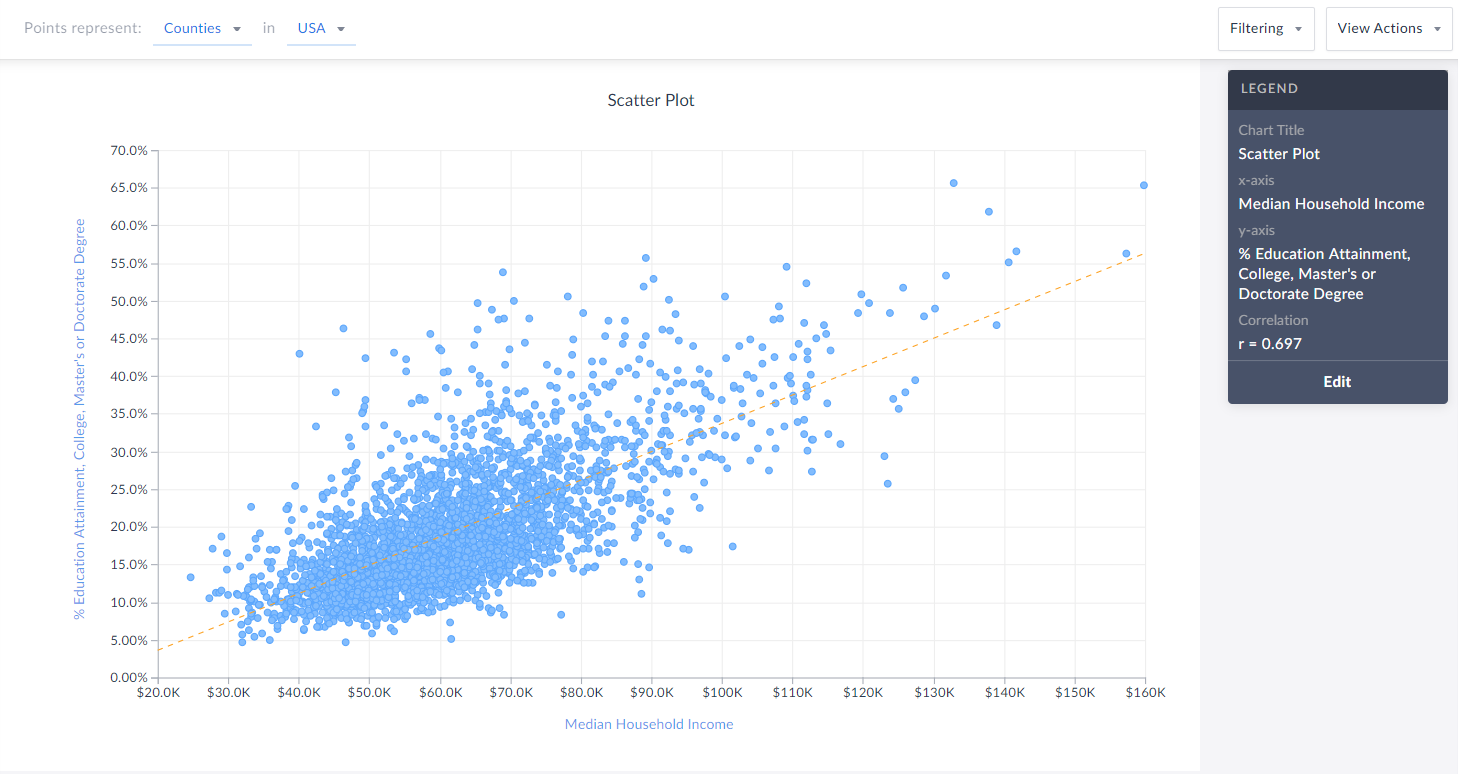
\includegraphics{class31_files/mediabag/income-vs-college.png}

}

\caption{Income vs Education}

\end{figure}%
\end{column}

\begin{column}{0.48\textwidth}
\begin{figure}[H]

{\centering 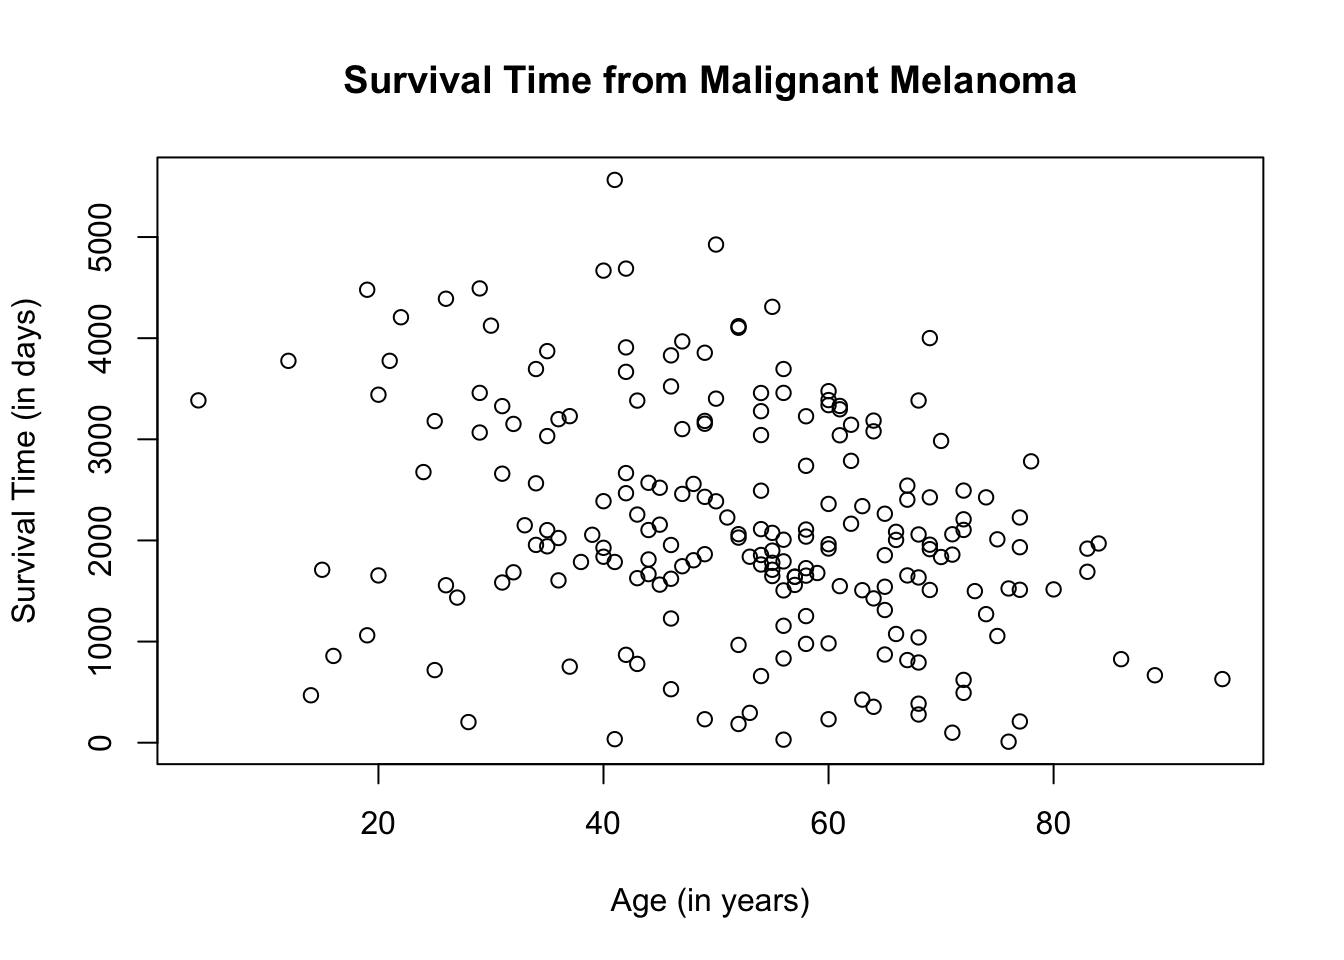
\includegraphics{class31_files/mediabag/age-vs-survival.png}

}

\caption{Age vs Survival}

\end{figure}%
\end{column}
\end{columns}
\end{frame}

\begin{frame}{Practice}
\phantomsection\label{practice}
Which image shows a \textbf{\emph{weak}} relationship between the
explanatory and response variables?

\begin{columns}[T]
\begin{column}{0.48\textwidth}
\begin{figure}[H]

{\centering 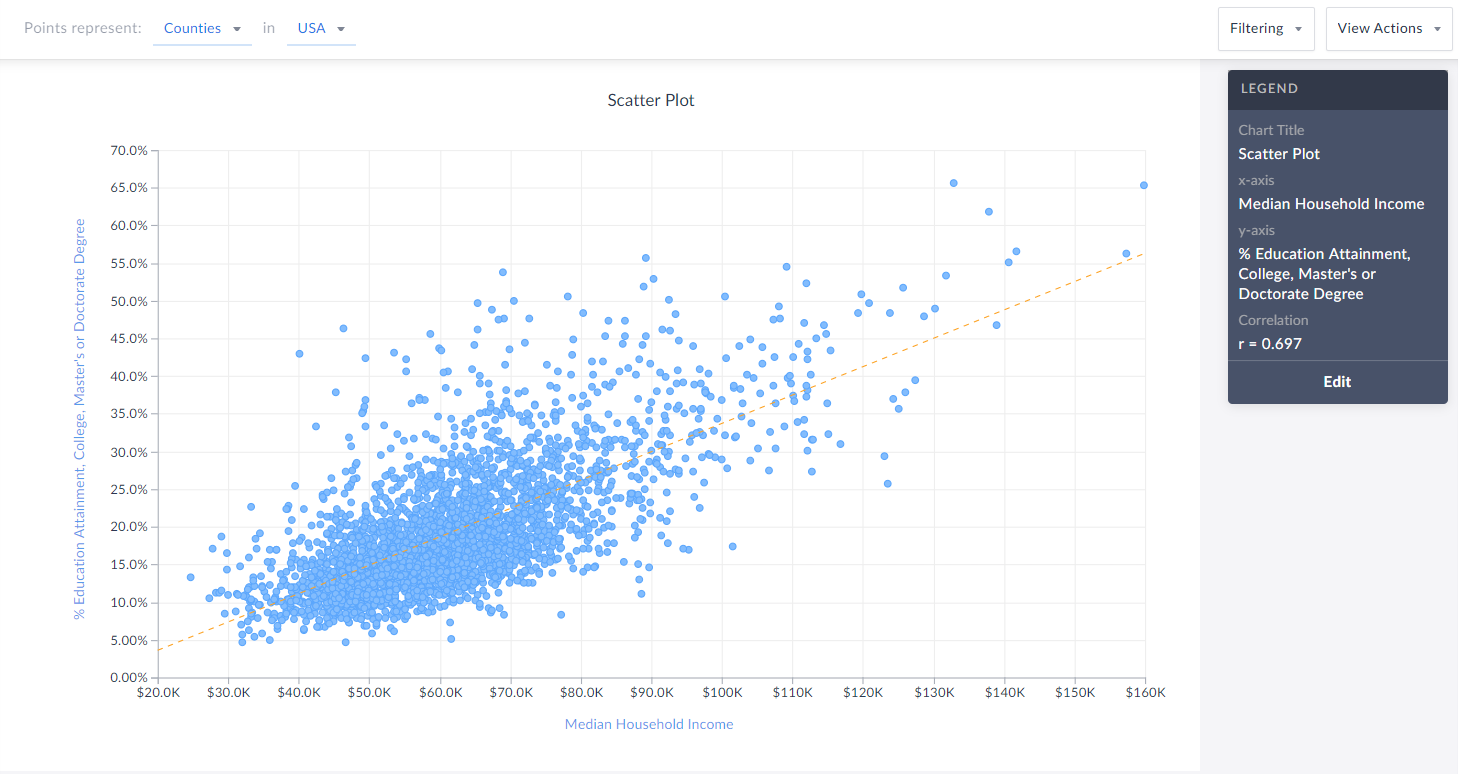
\includegraphics{class31_files/mediabag/income-vs-college.png}

}

\caption{Income vs Education}

\end{figure}%
\end{column}

\begin{column}{0.48\textwidth}
\begin{figure}[H]

{\centering 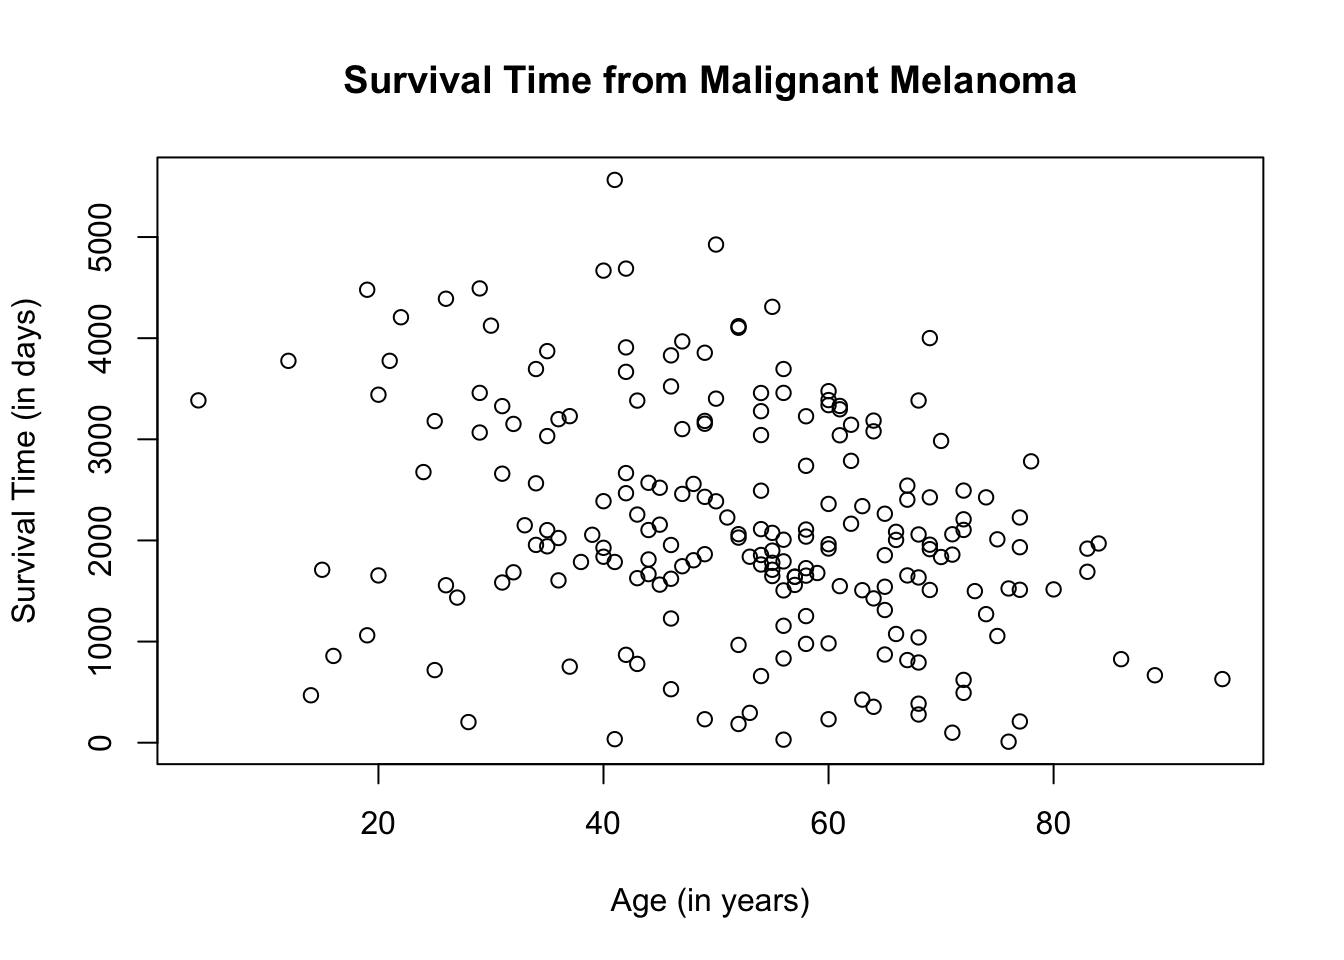
\includegraphics{class31_files/mediabag/age-vs-survival.png}

}

\caption{Age vs Survival}

\end{figure}%
\end{column}
\end{columns}
\end{frame}

\begin{frame}{Correlation}
\phantomsection\label{correlation}
\begin{itemize}
\tightlist
\item
  Describes the direction and strength of the association between 2
  numeric variables
\end{itemize}

\pause

\begin{itemize}
\item
  A correlation ranges from -1 to 1

  \begin{itemize}
  \item
    A perfect negative correlation equals -1
  \item
    A perfect positive correlation equals 1
  \end{itemize}
\end{itemize}

\pause

\begin{itemize}
\tightlist
\item
  A correlation of 0 indicates the two variables are independent (no
  relationship)
\end{itemize}

\pause

\begin{itemize}
\tightlist
\item
  We use the Pearson correlation for linear relationships
\end{itemize}
\end{frame}

\begin{frame}{Linear vs Non-Linear}
\phantomsection\label{linear-vs-non-linear}
\begin{center}
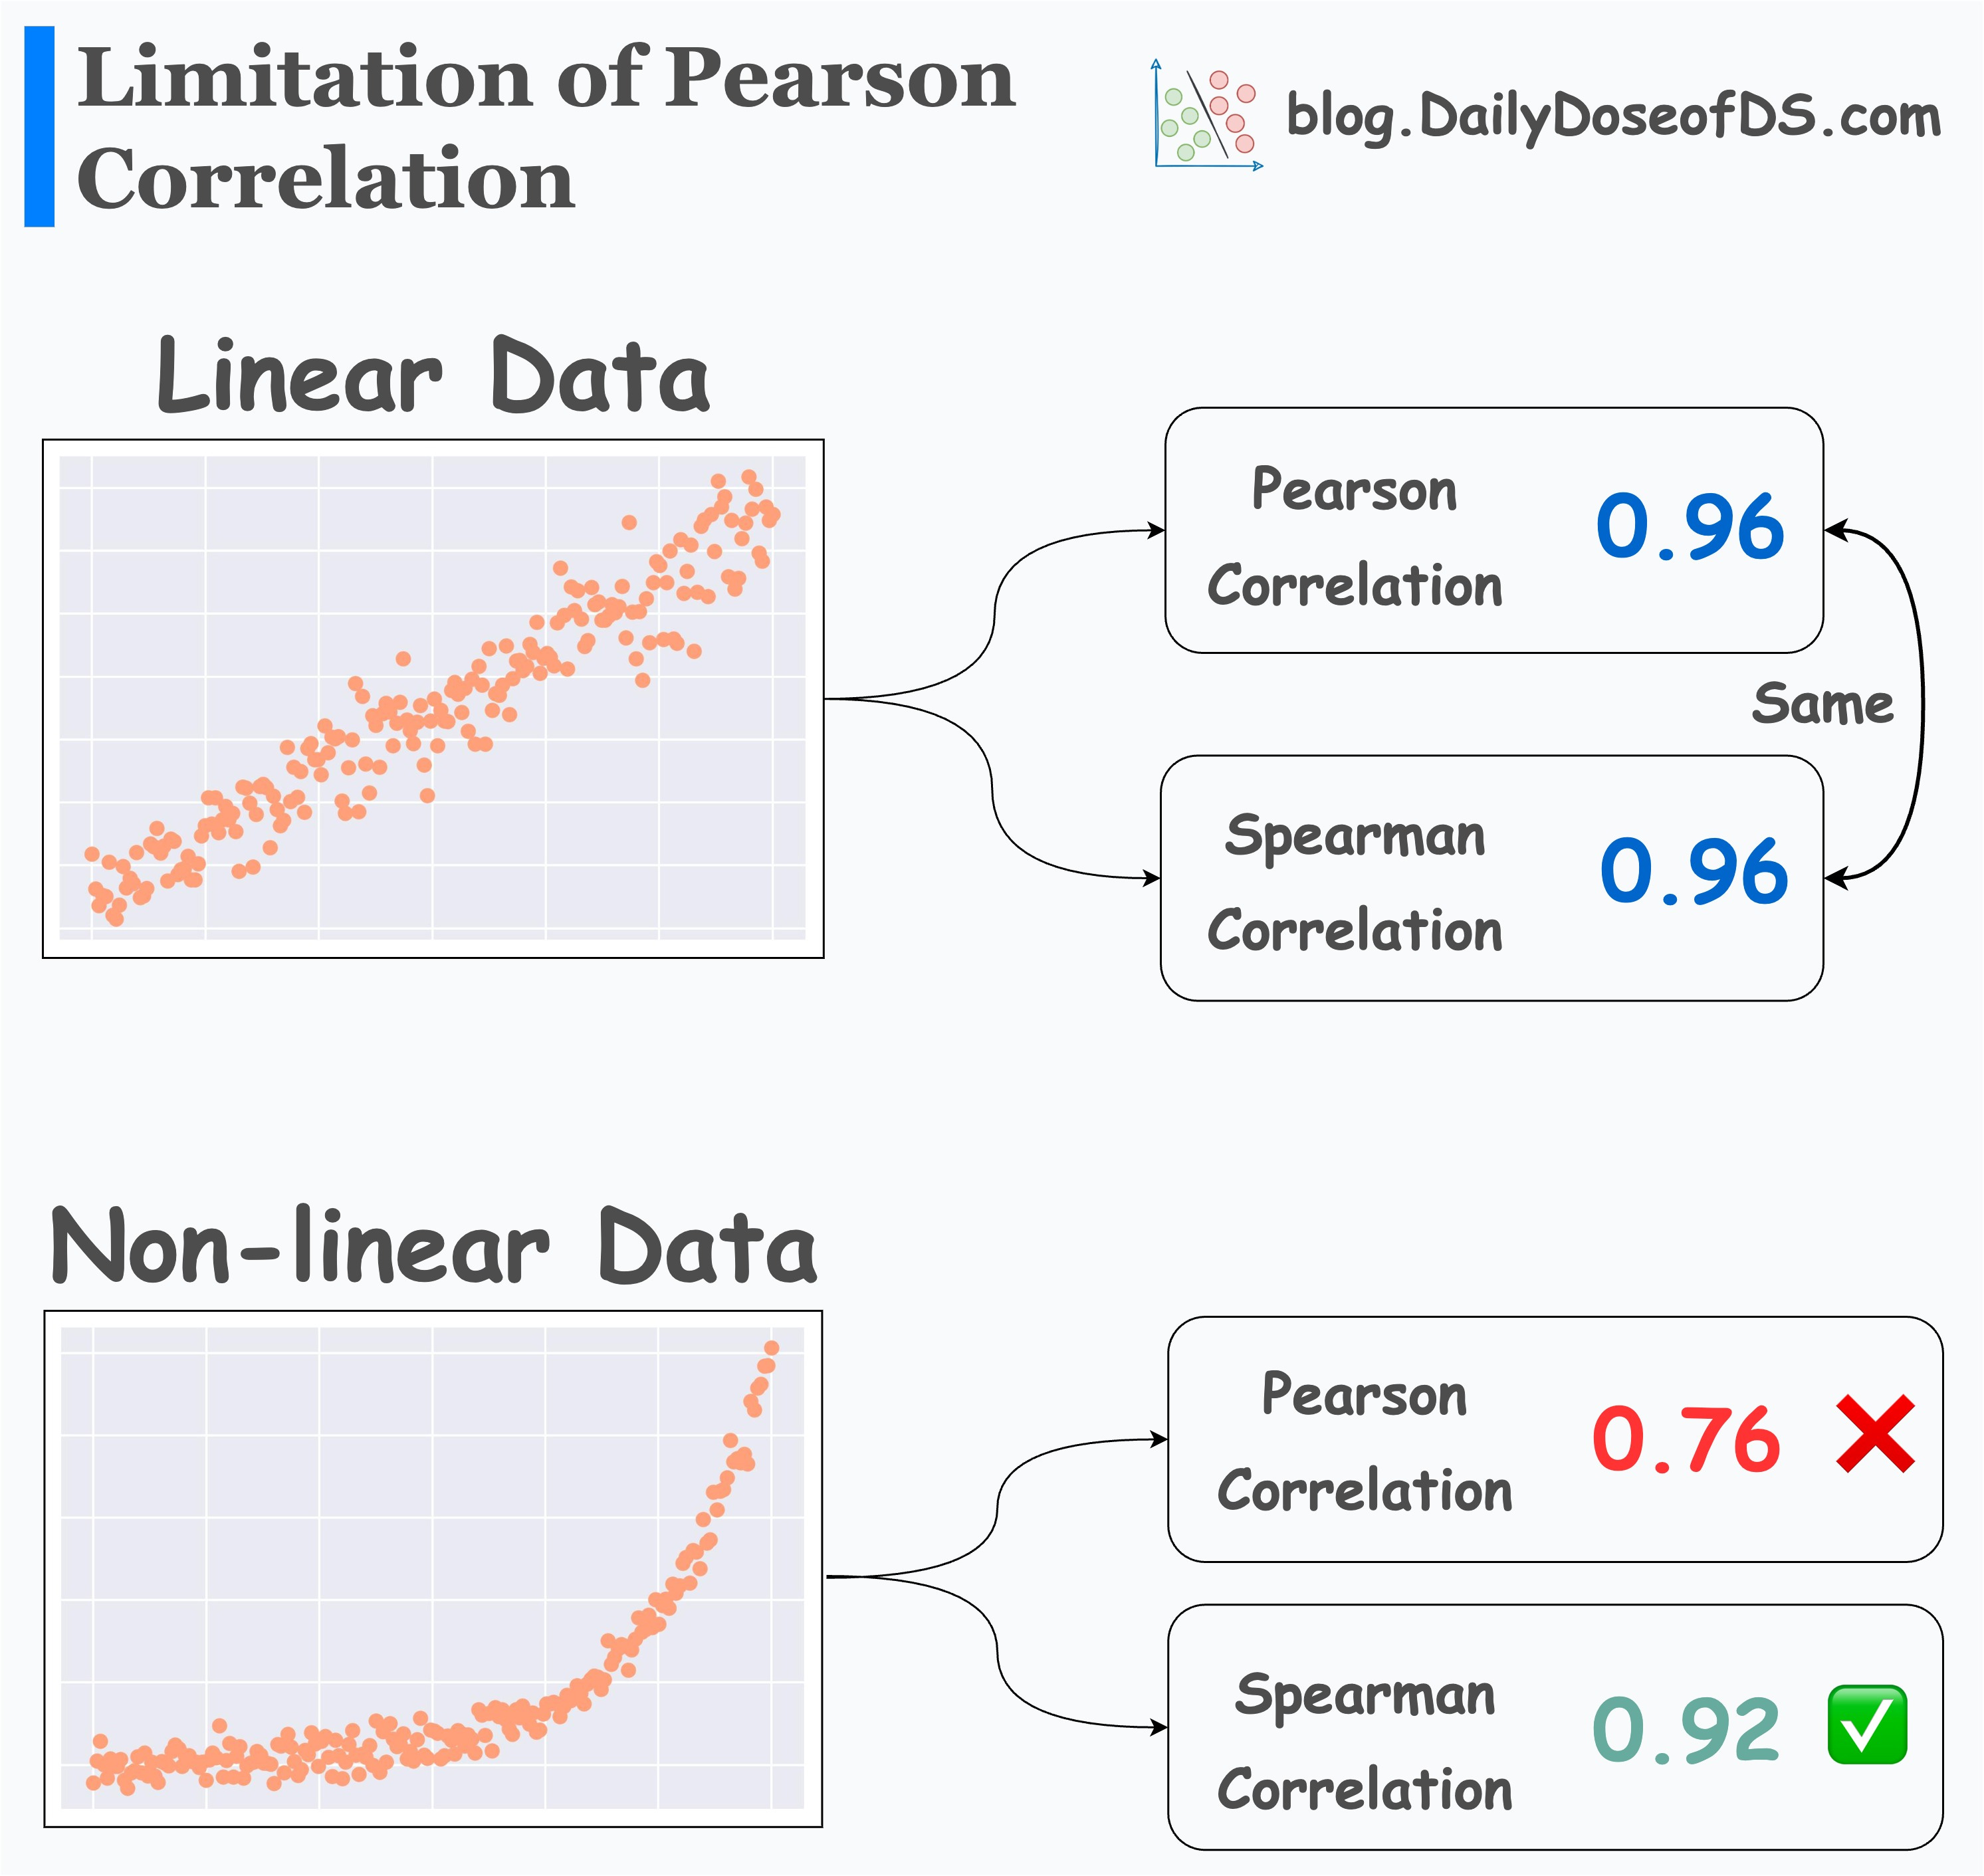
\includegraphics{class31_files/mediabag/linear-vs-nonlinear.jpg}
\end{center}
\end{frame}

\begin{frame}{Interpreting Correlations}
\phantomsection\label{interpreting-correlations}
\begin{center}
\includesvg{class31_files/mediabag/correlation-examples.svg}
\end{center}
\end{frame}

\begin{frame}{Example: Poverty vs Graduation Rate}
\phantomsection\label{example-poverty-vs-graduation-rate}
\begin{figure}[H]

{\centering 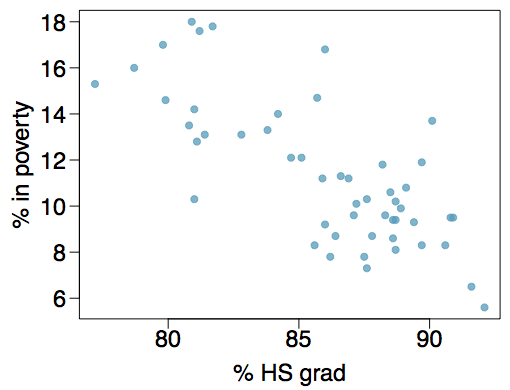
\includegraphics{class31_files/mediabag/poverty-vs-grad-rate.png}

}

\caption{What's the response variable?}

\end{figure}%

\pause

\textbf{\emph{Response Variable: Percent of people in poverty}}
\end{frame}

\begin{frame}{Example: Poverty vs Graduation Rate}
\phantomsection\label{example-poverty-vs-graduation-rate-1}
\begin{figure}[H]

{\centering 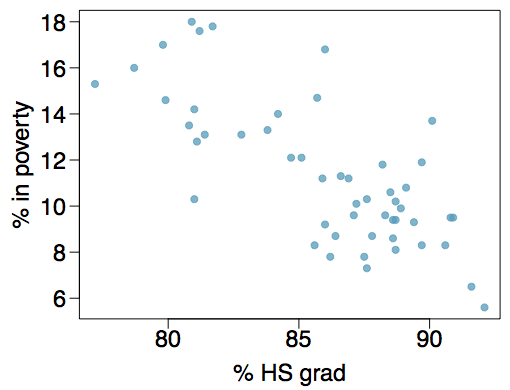
\includegraphics{class31_files/mediabag/poverty-vs-grad-rate.png}

}

\caption{What's the explanatory variable?}

\end{figure}%

\pause

\textbf{\emph{Explanatory variable: Percent of people who graduated high
school}}
\end{frame}

\begin{frame}{Example: Poverty vs Gradution Rate}
\phantomsection\label{example-poverty-vs-gradution-rate}
\begin{figure}[H]

{\centering 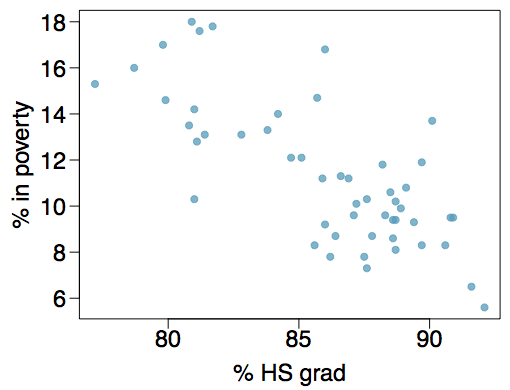
\includegraphics{class31_files/mediabag/poverty-vs-grad-rate.png}

}

\caption{Describe the relationship between these 2 variables.}

\end{figure}%

\pause

\textbf{\emph{Relationship: linear, negative, moderate to strong}}
\end{frame}

\begin{frame}{Example: Poverty vs Graduation Rate}
\phantomsection\label{example-poverty-vs-graduation-rate-2}
\begin{columns}[T]
\begin{column}{0.48\textwidth}
Which of the following is the most likely correlation? A) 0.60 B) -0.25
C) -0.75 D) 0.35
\end{column}

\begin{column}{0.48\textwidth}
\begin{figure}[H]

{\centering 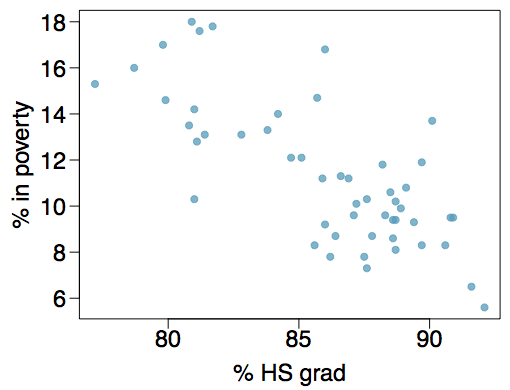
\includegraphics{class31_files/mediabag/poverty-vs-grad-rate.png}

}

\caption{Describe the relationship between these 2 variables.}

\end{figure}%
\end{column}
\end{columns}
\end{frame}

\begin{frame}{Example: Poverty vs Graduation Rate}
\phantomsection\label{example-poverty-vs-graduation-rate-3}
\begin{columns}[T]
\begin{column}{0.48\textwidth}
Which of the following is the most likely correlation?
\textbf{\emph{C.}} \textbf{\emph{-0.75}}
\end{column}

\begin{column}{0.48\textwidth}
\begin{figure}[H]

{\centering 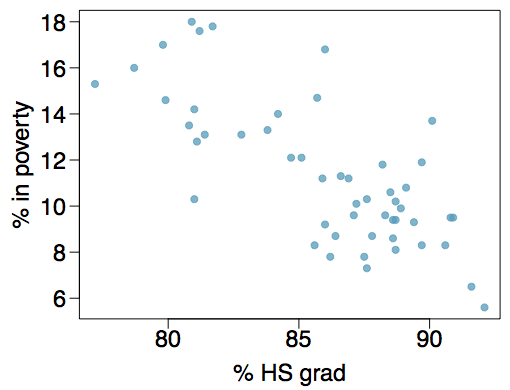
\includegraphics{class31_files/mediabag/poverty-vs-grad-rate.png}

}

\caption{Describe the relationship between these 2 variables.}

\end{figure}%
\end{column}
\end{columns}
\end{frame}

\begin{frame}{Testing a Correlation}
\phantomsection\label{testing-a-correlation}
\begin{itemize}
\tightlist
\item
  Null Hypothesis: The two variables are independent (correlation = 0)
\end{itemize}

\[
H_0 \colon \rho=0
\]

\pause

\begin{itemize}
\tightlist
\item
  Alternate Hypothesis: the two variables are dependent
\end{itemize}

\[
\begin{aligned}
H_A &\colon \rho > 0 \\
& \rho < 0 \\
& \rho \ne 0 \\
\end{aligned}
\]
\end{frame}

\begin{frame}{Test Statistic}
\phantomsection\label{test-statistic}
The test statistic \(t\) for the population Pearson correlation \(\rho\)
(Greek letter rho) is estimated using the observed correlation \(r\).

\[
t=\frac{r\sqrt{n-2}}{\sqrt{1-r^2}}
\]
\end{frame}

\begin{frame}[fragile]{Getting a p-value}
\phantomsection\label{getting-a-p-value}
Use the Student's \(t\) distribution with degrees of freedom
\(\text{df}=n-2\) to find a p-value for the observed correlation \(r\)
in a sample of size \(n\) under the null hypothesis
\(H_0 \colon \rho=0\).

\begin{Shaded}
\begin{Highlighting}[]
\CommentTok{\# specify the test statistic and degrees of freedom}
\FunctionTok{pt}\NormalTok{(test\_statistic,}
   \AttributeTok{df =}\NormalTok{ n}\DecValTok{{-}2}\NormalTok{,}
   \AttributeTok{lower.tail =}\NormalTok{ F) }\CommentTok{\# optional parameter}
\end{Highlighting}
\end{Shaded}
\end{frame}

\begin{frame}{Eyeballing a Line}
\phantomsection\label{eyeballing-a-line}
\begin{figure}[H]

{\centering 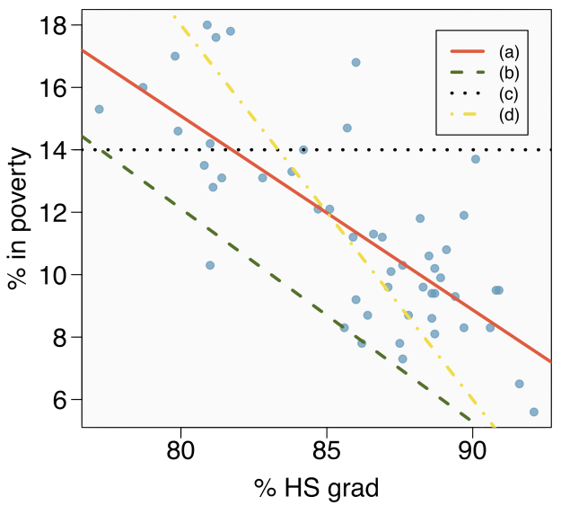
\includegraphics{class31_files/mediabag/eyeball-line.png}

}

\caption{How do we find the best line to draw through variables that
appear to have a linear relationship?}

\end{figure}%
\end{frame}

\begin{frame}{Quantifying Error: Residuals}
\phantomsection\label{quantifying-error-residuals}
\begin{figure}[H]

{\centering 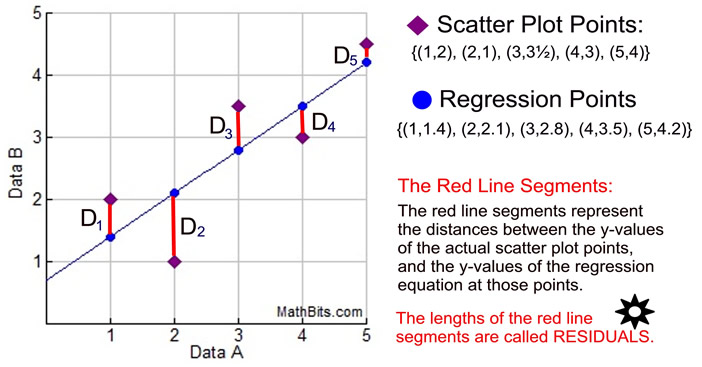
\includegraphics{class31_files/mediabag/residuals-example.jpg}

}

\caption{Residuals are the difference between the observed values and
the predicted values.}

\end{figure}%
\end{frame}

\begin{frame}{Special Topic: Correlation vs Causation}
\phantomsection\label{special-topic-correlation-vs-causation}
\begin{figure}[H]

{\centering 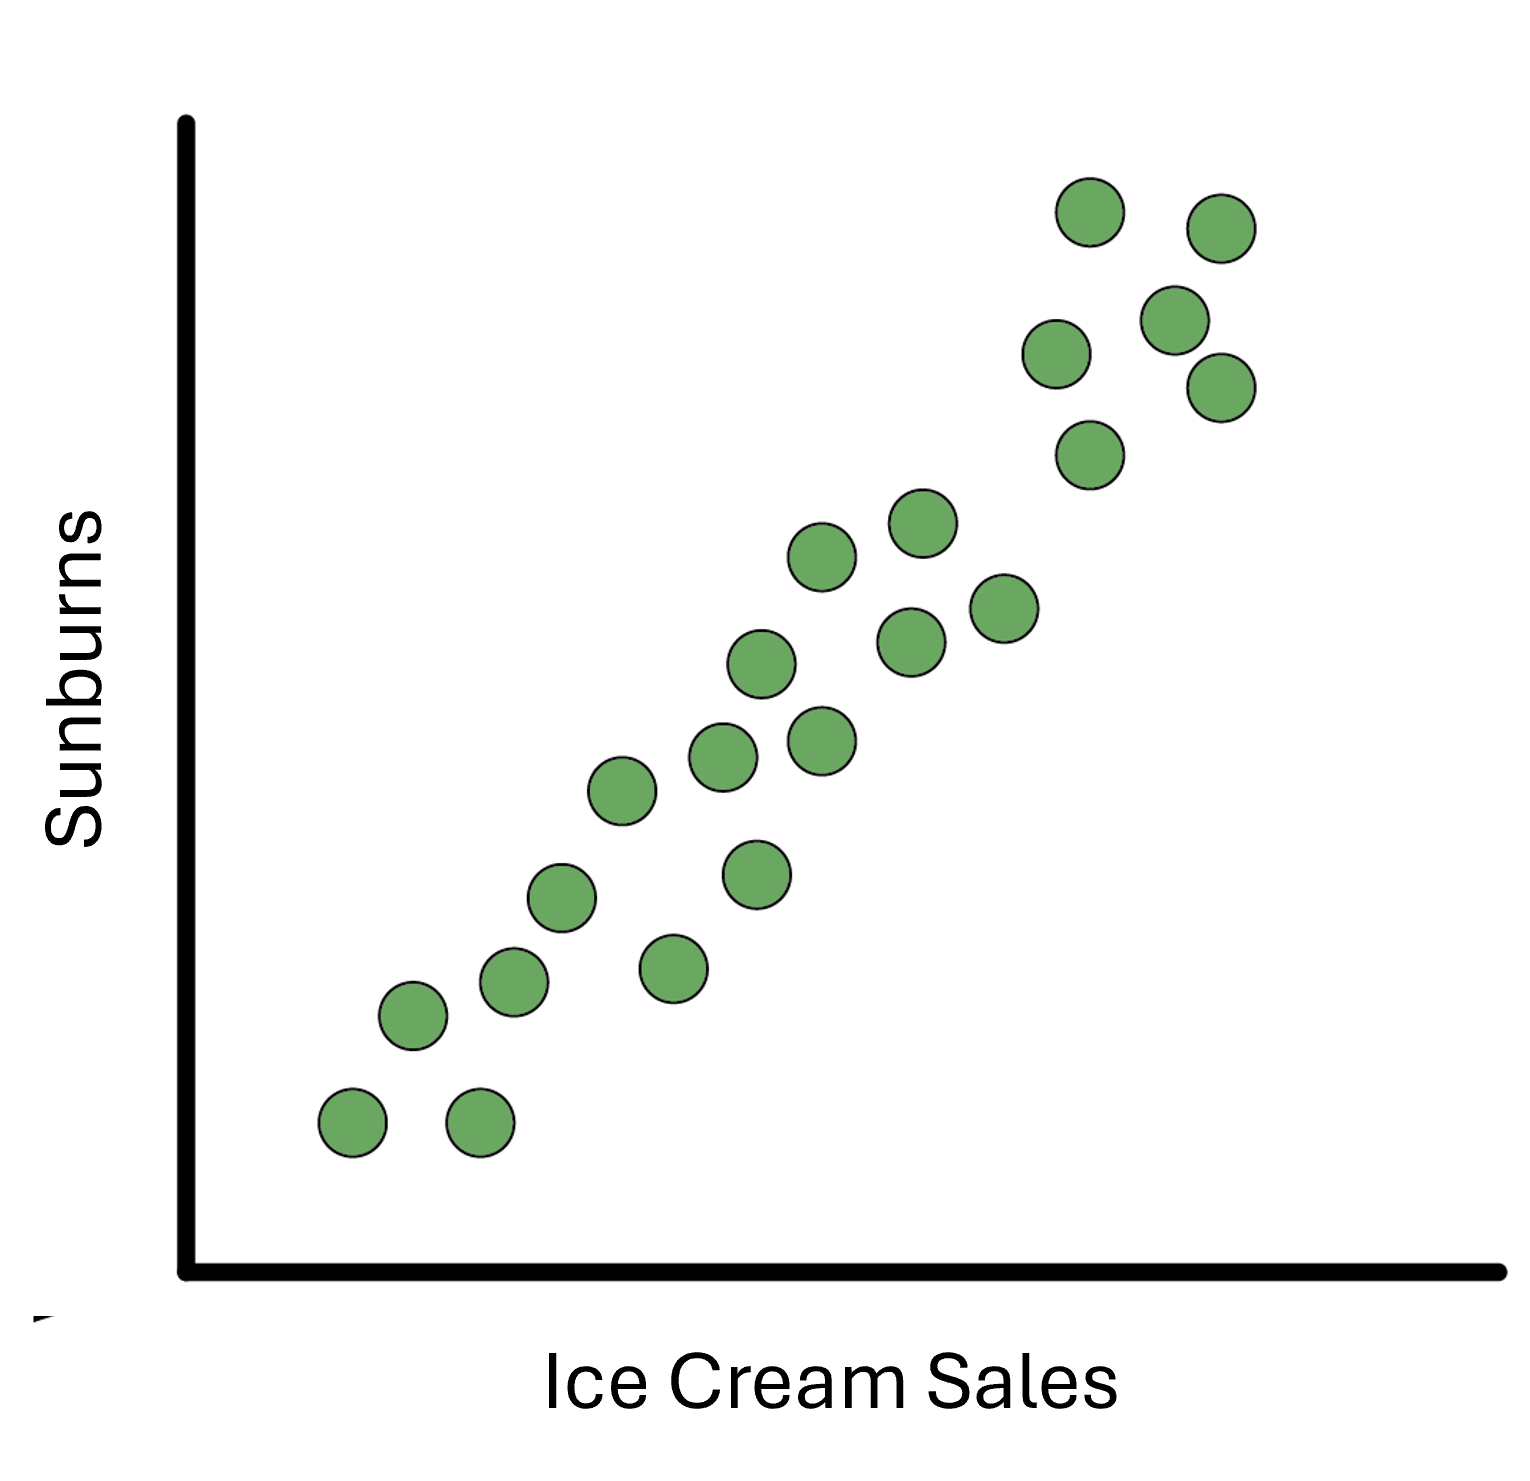
\includegraphics{class31_files/mediabag/ice-cream-sales.png}

}

\caption{Research Question: Do ice cream sales cause sunburns?}

\end{figure}%
\end{frame}

\begin{frame}{Special Topic: Correlation vs Causation}
\phantomsection\label{special-topic-correlation-vs-causation-1}
\begin{columns}[T]
\begin{column}{0.48\textwidth}
\begin{center}
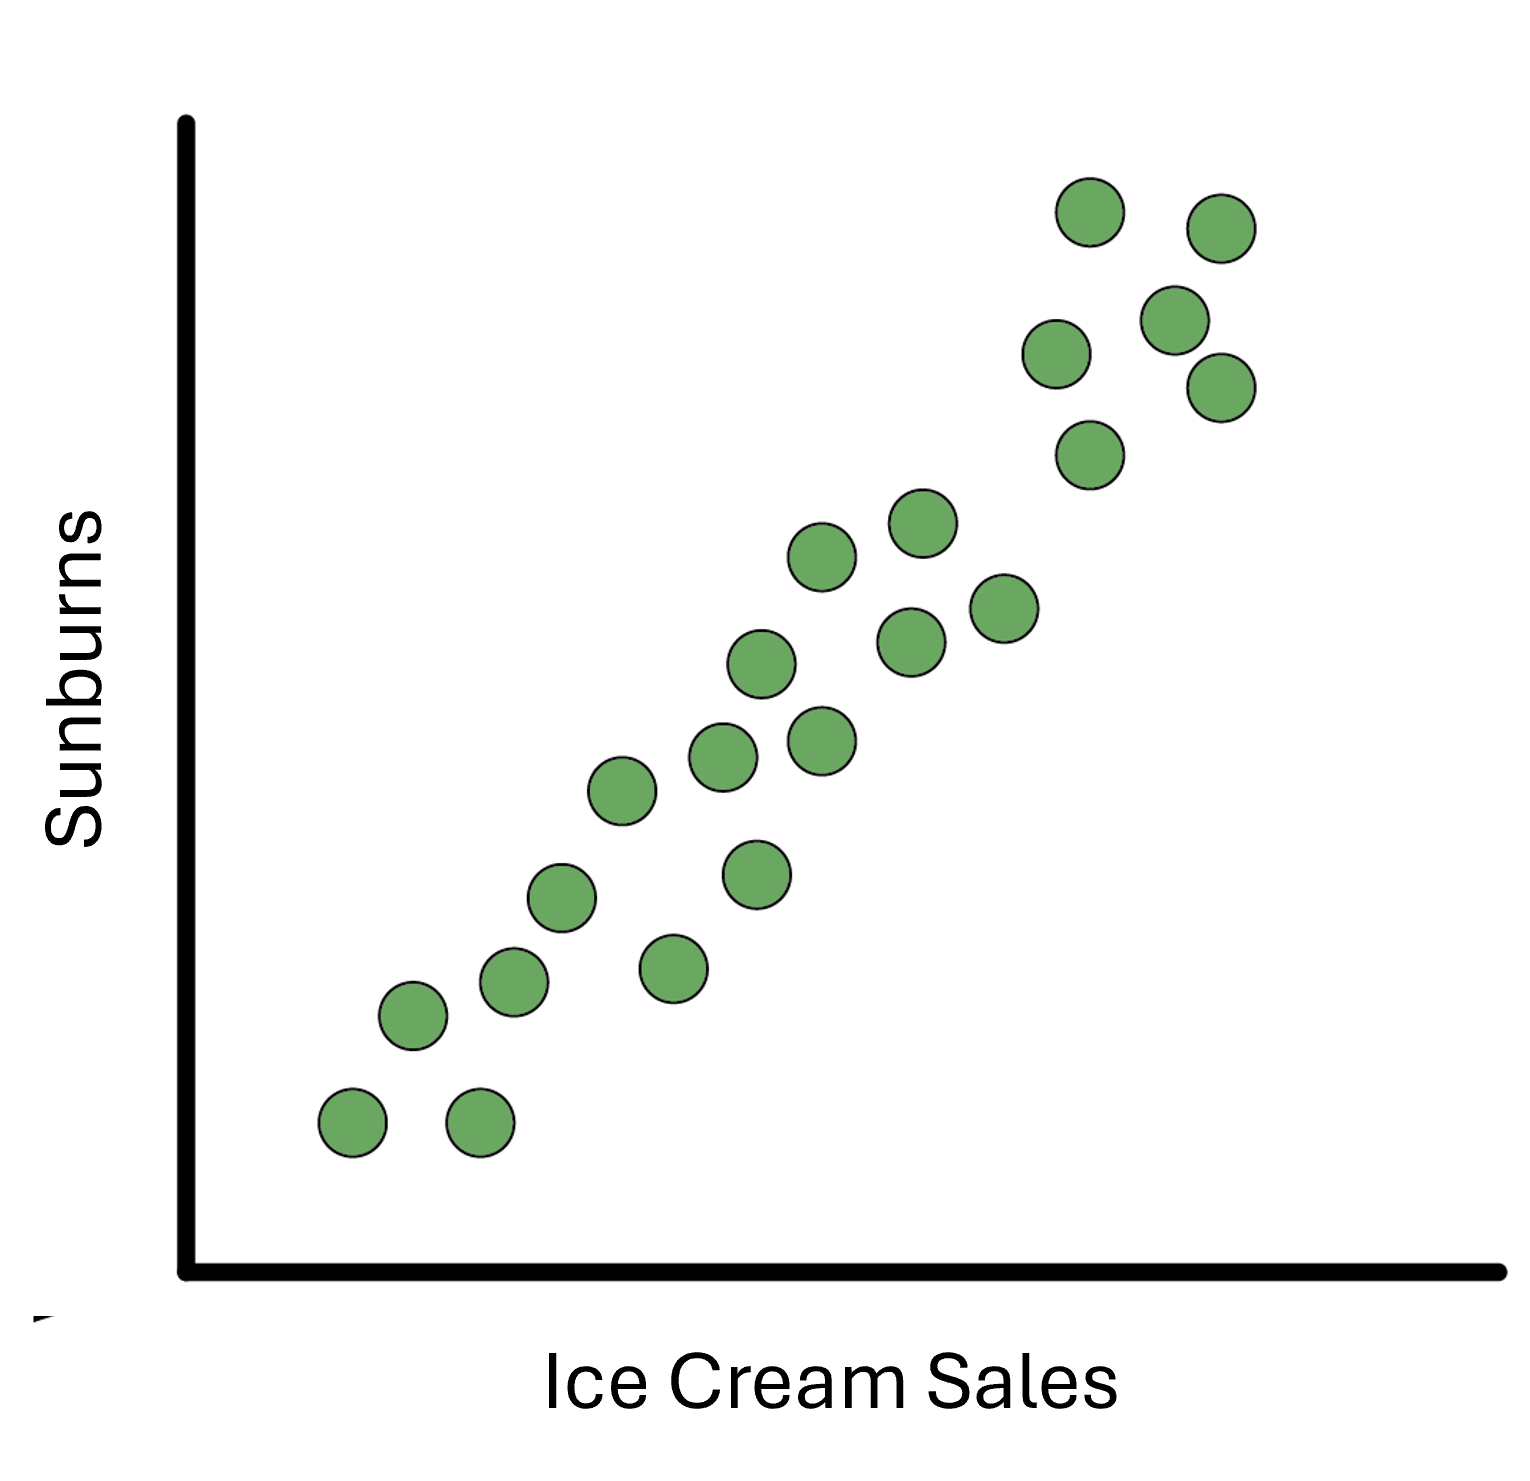
\includegraphics{class31_files/mediabag/ice-cream-sales.png}
\end{center}
\end{column}

\begin{column}{0.48\textwidth}
\begin{itemize}
\item
  As ice cream sales increase, the number of sunburns also increases
\item
  Strong, positive, linear correlation
\item
  High temperatures affect both ice cream consumption and behaviors that
  lead to sunburn
\end{itemize}
\end{column}
\end{columns}
\end{frame}

\begin{frame}{Confounding Variables}
\phantomsection\label{confounding-variables}
\begin{columns}[T]
\begin{column}{0.48\textwidth}
When you have a confounding variable, you might find dependence between
two unrelated variables that are only connected by the confounder.
\end{column}

\begin{column}{0.48\textwidth}
\begin{center}
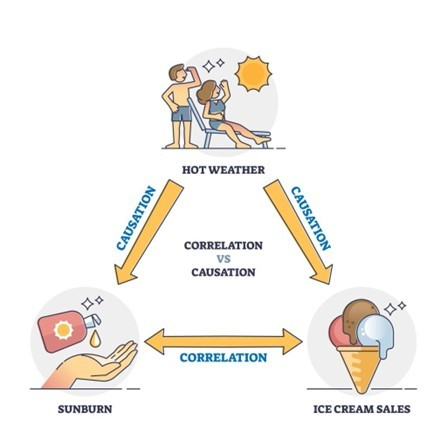
\includegraphics{class31_files/mediabag/confounders.jpg}
\end{center}
\end{column}
\end{columns}
\end{frame}




\end{document}
